\documentclass[11.5pt]{article}
\usepackage[utf8]{inputenc}
\usepackage[T1]{fontenc}
\usepackage[textwidth=460pt, top=80pt, bottom=80pt]{geometry}
\usepackage{graphicx}
\usepackage[justification=default]{subfig}
\usepackage[update]{epstopdf}
\usepackage[labelfont=bf]{caption}
\usepackage[dvipsnames]{xcolor}
\usepackage{fancyhdr}
\usepackage{booktabs}
\usepackage{multicol}
\usepackage{multirow}
\usepackage{titling}
\usepackage{float}
\usepackage{bm}
\usepackage[intlimits]{empheq}
\usepackage[hidelinks]{hyperref}
\usepackage{amsmath}
\usepackage{csquotes}
\usepackage{enumitem}
\usepackage{tikz}
\usetikzlibrary{positioning, 3d}
\usepackage{tabularx}

%Bibliography

\usepackage{csquotes}
\usepackage[
    sorting=none, %
    sortcites=true, %
    bibencoding=ascii, %
    autopunct=true, %
    hyperref=true, %
    language=auto, %
    %backref=true,%
    url=false, %
    %maxcitenames=10,%
    %minbibnames = 20,%
    maxbibnames=3, %
    giveninits,
    natbib=false,
    isbn=false, %
    backend=biber
]{biblatex}
\addbibresource{bibliography.bib}

\usepackage[]{hyperref}
\usepackage{cleveref}
%%% CREF setup
\crefname{equation}{Eq.}{Eqs.}
\crefname{table}{Table}{Tables}
\crefname{figure}{Fig.}{Figs.}

\begin{document}
    \begin{titlingpage}
        \begin{center}
            \begin{figure}
                \centering
                
\includegraphics[width=0.6\textwidth]{
                    graphics/logo.png
                }
            \end{figure}
            \Large{\textsc{Politecnico di Milano}}
            \vspace{1cm}
            \rule{0.95\textwidth}{0.7mm}
            {\Large{\textbf{Requirement Engineering and Design Project:\\ SustainCity \\ V 1.0.1}}}
            \rule{0.95\textwidth}{0.7mm}
            \vspace{1cm}
            \large{Prof. Elisabetta Di Nitto \\ A.Y. 2024-2025}
            \vspace{1cm}

            \large{Authors: \\ \textbf{Riccardo Donati, Camilo Martínez, Jialiclaudio Huang, Peng Rao}}

            \vspace{1cm}
            
            \text{Last update: \today}
            % \large{Authors: \\ \textbf{Peng Rao} (ID 270661)}
        \end{center}
    \end{titlingpage}

    \pagenumbering{roman}

    \tableofcontents

    \clearpage

    \setcounter{page}{1}
    \pagenumbering{arabic}

    \section{The project and project goals}
    \subsection{Problem Statement}
    Urban commuting is a major contributor to environmental degradation and climate change due to air pollution and greenhouse gas emissions. To address this issue, the \textbf{SustainCity} project aims to develop a smart traffic management system that optimizes urban mobility through real-time adjustments and long-term strategic planning.

    To reduce the impact of urban commuting, we want to keep it under control with the following types of actions: 
    \begin{enumerate}
        \item \textbf{Dynamically adjusts traffic lights (Type1)} based on real-time sensor data to minimize congestion.
        \item \textbf{Analyzes historical traffic patterns (Type2)} to recommend structural optimizations (e.g., one-way streets, bus schedule adjustments).
        \item \textbf{Automatically adapts to planned events (Type3)} by preemptively reconfiguring traffic flows and public transport routes.
        \item \textbf{Provides transparent reporting} to citizens and policymakers on traffic interventions and their environmental benefits.
    \end{enumerate}

    \subsection{Goal and approach}
    In this project, we aim to put into practice the concepts learned in the first part of the Software Engineering for HPC course. We will analyze the problem outlined, and document our findings and proposed solutions. Our report will cover the following key aspects.
    \begin{itemize}
        \item Requirement Analysis: We will identify and extract use cases, functional and non-functional requirements, and domain assumptions based on the problem statement.

        \item Architectural Design: We will define a system architecture using component diagrams and sequence diagrams to illustrate the system’s structure and interactions. Sequence diagrams will highlight how components interact with one another. We will discuss potential critical challenges in our system and propose strategies to address them.
    \end{itemize}

    \subsection{Stakeholders}
    \begin{itemize}
        \item \textbf{Urban Traffic Managers}: Approve and implement Type2 \& Type3 recommendations.
        \item \textbf{Public Transport Operators}: Adjust schedules based on system insights.
        \item \textbf{Citizens}: Access reports to understand traffic policies and environmental impact.
    \end{itemize}

    \section{Requirement analysis}
    \subsection{Relevant human and non-human actors}
    \subsubsection{Human Actors}
        \begin{itemize}
        \item \textbf{Urban Area Managers}
        Approve or reject proposed traffic optimizations.
        Oversee traffic management and policy decisions.
        \item \textbf{Citizens}
        Access daily and yearly reports on traffic adjustments. 
        Stay informed about the city's traffic management.
        \end{itemize}
    \subsubsection{Non-Human Actors}
    \begin{itemize}
        \item \textbf{Traffic Sensor System}
    Collects real-time traffic data and publishes it on the message bus.
    Publishes congestion levels to the event-driven infrastructure.
    \item \textbf{Public Transport System (Microservice)}
    Provides schedule data for buses and public transport lines.
    Assists in traffic analysis and optimization planning.
    \item \textbf {News Channel}
    Publishes real-time event announcements that may impact traffic.
    \item \textbf{Events}
    Events represent significant occurrences (e.g., concerts, sports events, festivals) that influence traffic flow and public transport in the city.
    \end{itemize}
    
    \subsection{Use cases}
    \subsubsection{Type1}
    \begin{table}[!htp]
        \centering
        \begin{tabular}{@{} l p{23em} @{}}
            \toprule \multicolumn{2}{c}{Use Case: \textbf{Modify Traffic Lights}} \\
            \midrule                                                                          %%%
            Actors                                                                           &  Traffic Sensor System, Citizens \\
            %%%
            Entry condition                                                                  &  Traffic congestion is detected through real-time analysis, requiring traffic light adjustments.\\
            %%%
            Flow of Events                                                                   & \begin{enumerate}[left=0pt, parsep=0pt, topsep=0pt]
            \item System receives traffic data from the Traffic Sensor System.
            \item A new light timing configuration is generated based on congestion analysis.
            \item Updated timings are sent to the Traffic Light Controller.
            \item The controller applies the changes and confirms success.
            \item Changes are logged via the Logging Service.
            \item The Report Generator retrieves logs daily and creates a report including Type 1 actions.
            \end{enumerate} \\
            %%%
            Exit condition                                                                   &  New traffic light durations are applied and confirmed. \\
            %%%
            Exceptions                                                                       &  \begin{enumerate}[left=0pt, parsep=0pt, topsep=0pt]
            \item Communication failure when retrieving or applying the configuration.
            \item Invalid configuration (e.g., unsafe green light duration).
            \item Logging service is unavailable.
            \end{enumerate} \\
            Special Requirements                                                             & \begin{enumerate}[left=0pt, parsep=0pt, topsep=0pt]
            \item All changes must be securely logged
            \item Communication must be encrypted.
            \item System must operate with high availability and near real-time response.
            \end{enumerate} \\
            \bottomrule
        \end{tabular}
        \caption{Detailed use case Modify Traffic Lights.}
        \label{Use Case - Research Trip}
    \end{table}
    \subsubsection{Type2}
    \begin{table}[!htp]
        \centering
        \begin{tabular}{@{} l p{23em} @{}}
            \toprule \multicolumn{2}{c}{Use Case: \textbf{Dynamic Traffic Light Adjustments}} \\
            \midrule                                                                          %%%
            Actors                                                                           &  \\
            %%%
            Entry condition                                                                  &  \\
            %%%
            Flow of Events                                                                   &  \\
            %%%
            Exit condition                                                                   &  \\
            %%%
            Exceptions                                                                       &  \\
            Special Requirements                                                             &  \\
            \bottomrule
        \end{tabular}
        \caption{Detailed use case explanation - Research Trip.}
        \label{Use Case - Research Trip}
    \end{table}

    \newpage
    
    \subsubsection{Event-Specific Traffic Configuration(Type 3)}
    This use case details how the \textbf{SustainCity system} collects information about planned large crowd events and defines event-specific configurations for traffic lights, roads and public transport schedules. 

    \begin{table}[H]
        \centering
        \begin{tabular}{@{} l p{23em} @{}}
            \toprule \multicolumn{2}{c}{Use Case: \textbf{Define Event-Specific Traffic Configurations}} \\
            \midrule   
            \textbf{Actors} & News Channel, SustainCity System, Urban Area Managers \\
            \textbf{Entry condition} & A planned event (e.g., concert, sports game) is announced via the news channel. \\
            \textbf{Flow of Events} & 
            \begin{enumerate}[left=0pt, parsep=0pt, topsep=0pt]
              \item The system receives an event notification from the city news channel.
              \item It extracts key details: type, location, timing, and expected attendance.
              \item Affected streets and areas are identified.
              \item Public transport schedules for those areas are retrieved via the microservice.
              \item Recent and historical traffic data is analyzed.
              \item Based on the analysis, the system generates event-specific configuration suggestions:
              \begin{itemize}
                \item Adjust traffic lights
                \item Modify road directions
                \item Update public transport schedules
              \end{itemize}
              \item Suggestions are sent to urban area managers.
              \item All suggestions and their acceptance status are logged for reporting.
            \end{enumerate}
             \\
            \textbf{Exit condition} & Event-specific traffic configurations are implemented or rejected. \\
            \textbf{Exceptions} & 
            \begin{itemize}[left=0pt, parsep=0pt, topsep=0pt]
                \item News Channel Feed is unavailable: The system attempts to reconnect to the News Channel Feed every 5 minutes.
                \item Event attendance significantly exceeds predictions: The system triggers an emergency traffic pattern reconfiguration
            \end{itemize} \\
            \textbf{Special Requirements} & 
            \begin{itemize}[left=0pt, parsep=0pt, topsep=0pt]
                \item System must respond to event notifications in near real-time.
                \item Generated suggestions must be traceable for yearly reporting.
                \item Suggestions must be explainable and visualizable for city officials.
            \end{itemize} \\
            \bottomrule
        \end{tabular}
    \end{table}
    \subsection{Domain assumptions}
    \begin{enumerate}
        \item The sensors present accurate data.
        \item The microservice is accessible at all times.
        \item The microservice is always updated.
        \item Public transport is always reasonably on time.
        \item The news channel publishes the news early enough to have time for the decision making process.
        \item The news channel provides enough information for the decision making process to take place.
        \item The urban area managers make decisions quickly enough to ensure changes align with the ongoing situation.
        \item The system controls traffic lights in real time.
        \item Users and drivers receive accurate notifications.
    \end{enumerate}
    \subsection{Requirements}
    \subsubsection{Functional requirements}
    \paragraph{Type 1:}
    \begin{enumerate}
        \item The system shall receive real-time traffic data from the Traffic Sensor System.
        \item The system shall analyze traffic flow patterns to detect congestion.
        \item The system shall modify traffic light durations dynamically based on traffic flow. For instance, if traffic on a specific road is significantly higher than on intersecting roads, the system shall extend the green light duration for the busy road and extend the red light duration for the other roads.
        \item The system shall log all traffic light modifications on a daily basis.
        \item The system shall generate daily reports summarizing traffic flow and
            Type 1 actions taken, including any changes to light durations.
        \item The system shall make traffic reports accessible to citizens via a
            digital platform (e.g., website or mobile app).
    \end{enumerate}

    \paragraph{Type 2:}
    \begin{enumerate}
        \item The system shall collect and analyze historical traffic data to identify
            trends and recurring congestion patterns.

        \item The system shall propose optimizations for one-way street configurations
            where applicable to improve traffic flow.

        \item The system shall propose optimizations for traffic light configurations.

        \item The system shall propose optimizations for public transport schedules
            (e.g., adding buses or adjusting bus frequencies during peak times).

        \item The system shall allow Urban Area Managers to approve or reject suggested
            optimizations.

        \item The system shall log all accepted and rejected optimization proposals.
    \end{enumerate}
    \paragraph{Type 3:}
    \begin{enumerate}
        \item The system shall receive event announcements from the News Channel.

        \item The system shall analyze the impact of each event based on location,
            time, and expected attendance to assess the potential effect on traffic
            and public transport.

        \item The system shall propose event-specific traffic and public transport adjustments (e.g., rerouting roads, adjusting public transport schedules).

        \item The system shall allow Urban Area Managers to approve or reject event-specific
            adjustments.

        \item The system shall log all accepted and rejected event-based changes.
    \end{enumerate}
    \subsubsection{Non-functional requirements}
    \begin{enumerate}
        \item The system shall process and analyze real-time traffic data within 10 seconds of receiving it.
        \item The system shall update traffic light configurations within 30 seconds of detecting congestion.
        \item The system shall be operational 24/7.
        \item The system shall support data input from at least 500 traffic sensors simultaneously.
        \item The system shall handle up to 50 event announcements per day without performance degradation.
        \item The system shall ensure that only authorized Urban Area Managers can approve or reject suggestions.

    \end{enumerate}
    \section{Design}
    \subsection{General description of the architecture}
    \subsection{Sequence diagrams}
    \subsubsection{Type1}
    Description of the main elements of the Type1 sequence diagram:
    \begin{enumerate}
        \item Participants
        \begin{itemize}
        \item Traffic Sensor System (TSS): Represents the sensor infrastructure that collects real-time traffic data.  
        \item Traffic Management System (TMS): It is the central system that processes the data from the sensors. It is responsible for analyzing traffic flow, detecting congestion, and deciding actions for adjusting traffic light timings. It also manages some statistics for reporting purposes.
        \item Traffic Light Controller (TLC): It is the controller for managing the traffic lights. Once the TMS determines if an action of adjusting traffic light durations is needed, it sends instructions to the TLC. The controller then updates the lights configuration and confirms the update back.
        \item Logging Service: It is responsible for logging any changes made to traffic light durations.
        \item Report Generator: It fetches the necessary logs and stats from the TMS and generates the reports. This includes daily statistics on traffic flow and the actions taken by the system.
        \item Citizen Platform: Provides access to traffic reports for citizens.
    \end{itemize}

    \item Interactions
        \begin{itemize}
        \item publishTrafficData(): The Traffic Sensor System sends real-time traffic data to the Traffic Management System (TMS).
        \item analyzeTrafficFlow(): The TMS processes the received traffic data. This step involves analyzing the flow of traffic, calculating statistics like vehicle counts, wait times, and traffic density.
        \item evaluateCongestionPatterns(): After analyzing traffic flow, the TMS evaluates the data to detect congestion patterns. For example, if the traffic density exceeds a predefined threshold, the system decides whether action is needed, such as extending green lights.
        \item updateLightConfig(roadId, newConfig): Based on the congestion patterns, the TMS instructs the Traffic Light Controller (TLC) to update the duration of the traffic lights on specific roads. For example, it may decide to extend the green light on a busy road.
        \item confirmUpdate(): The TLC confirms that the traffic light timings have been updated successfully.
        \item logAction(updatedDetails): The TMS logs the change details to the Logging Service.
        \item fetchLogs(): The Report Generator fetches the logs from the Logging Service to gather all recorded actions for that day.
        \item getTrafficStats(): The Report Generator retrieves the necessary traffic statistics from the TMS. 
        \item generateDailyStats(): The Report Generator processes the logs and stats to generate the daily traffic report about the average traffic flow on the main roads.
        \item displayDailyReport(): The Report Generator publishes the daily report to the Citizen Platform, where it is made available for public viewing.
    \end{itemize}
    \end{enumerate}
    \subsubsection{Type2}

    \newpage
    
    \subsubsection{Type3}
    \begin{figure}[htbp]
        \centering
        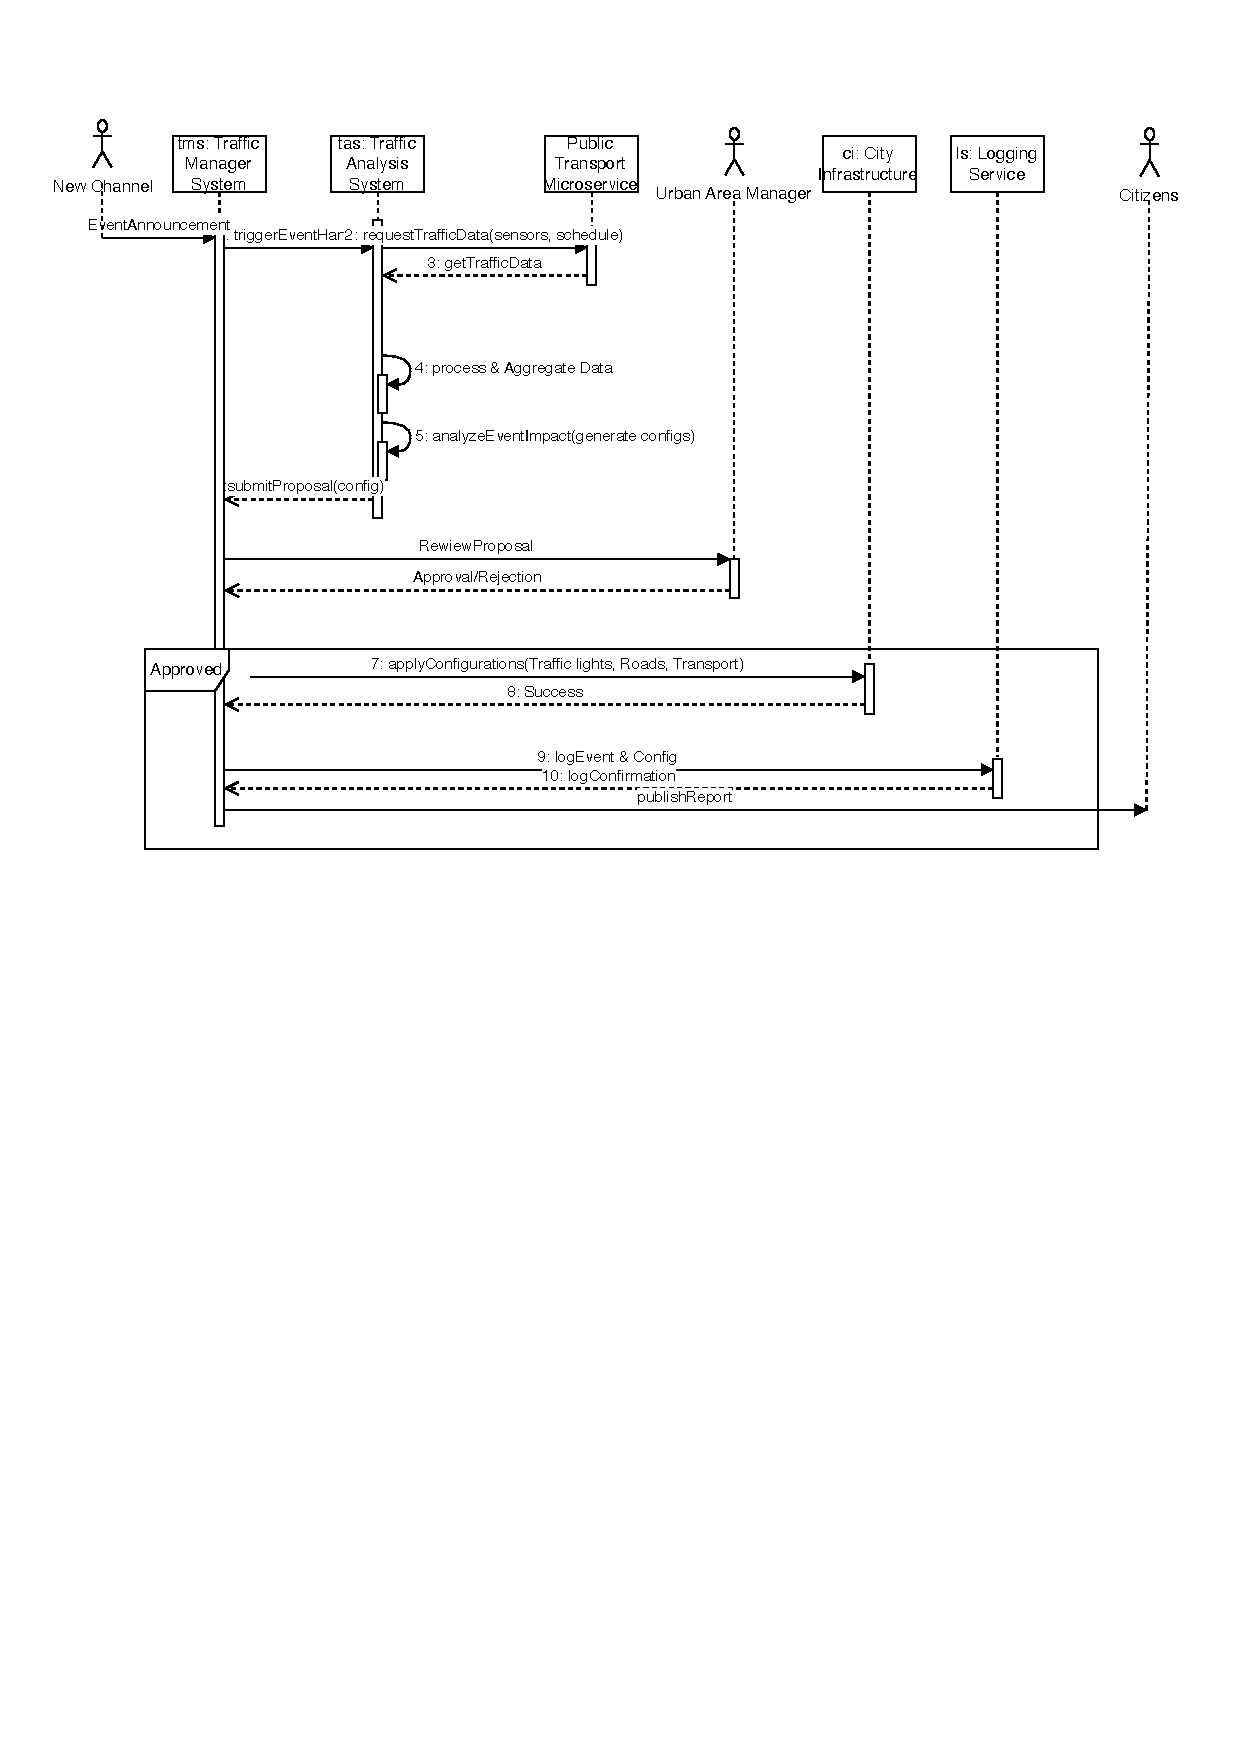
\includegraphics[width=0.9\textwidth]{figures/sequence-diagram-type3.pdf}
    \end{figure}
    \par{Participants:}
    \begin{itemize}
        \item \textbf{News Channel}: Publishes event announcements (e.g., concerts, sports events) as soon as they are planned.
        \item \textbf{Traffic Management System}: The central system managing the entire process.
        \item \textbf{Traffic Analysis System}: Responsible for data processing and traffic impact analysis.
        \item \textbf{Public Transport Microservice}: Provides real-time data from public transport (buses, metros, etc.).
        \item \textbf{Urban Area Managers}: Responsible for reviewing and approving proposed traffic plans.
        \item \textbf{City Infrastructure}: The actual infrastructure (e.g., traffic lights, roads) that will apply changes.
        \item \textbf{Logging Service}: Stores logs of events and configurations.
    \end{itemize}
    The main interactions could be as follows:
    \begin{enumerate}
        \item \textbf{Event Announcement}. News Channel $\rightarrow$ Traffic Management System: Sends EventNotification(eventDetails) (asynchronous message). The news channel transmits event details (e.g. location, time, expected crowd size).
        \item \textbf{Fetch Public Transport Data}. 
        \begin{itemize}
            \item Traffic Analysis System $\rightarrow$ Public Transport Microservice: Calls getScheduleByStreet(streetName) (synchronous).
            \item Public Transport Microservice $\rightarrow$ Traffic Analysis System: Returns ScheduleData.
        \end{itemize}
        \item \textbf{Generate Configuration Plan}. Traffic Analysis System $\rightarrow$ Traffic Analysis System: GenerateConfigurationPlan() (self-message). Processes event data and transport schedules to create traffic light adjustments, road changes, and public transport updates.
        \item \textbf{Suggest Configuration to Managers} Traffic Analysis System $\rightarrow$ Urban Area Managers: Sends SuggestConfiguration(configurationPlan). Proposes event-specific changes (e.g., extend green lights on main routes, set one-way roads).
        \item \textbf{Manager Approval}. Urban Area Managers $\rightarrow$ Traffic Management System: Sends ApprovalResponse(approved). Managers review and approve the plan (assumed approval for this flow).
        \item \textbf{Apply Traffic Light Configurations}. Traffic Management System $\rightarrow$ City Infrastructure: Sends ApplyTrafficLightConfig(config).
        \item \textbf{Log Action and Update Reports}. Traffic Manager System $\rightarrow$ Logging Service: Sends LogType3Action(config, "Applied"). Records the action for yearly reports and citizen notifications.
    \end{enumerate}
    
    \subsection{Critical Points and Design Decisions}
    This section outlines the key challenges faced during the system design and the corresponding decisions to address them.    
    \begin{itemize}
        \item \textbf{Real-Time Processing Latency}
        \begin{itemize}
            \item \textit{Criticality}: Type1 actions require immediate traffic light adjustments. Delays could worsen congestion.
            \item \textit{Decision}: Implemented Apache Kafka for stream processing and co-located edge servers near sensors.
            \item \textit{Trade-off}: Increased infrastructure costs but ensured sub-second response times.
        \end{itemize}
        
        \item \textbf{Legacy System Integration}
        \begin{itemize}
            \item \textit{Criticality}: Heterogeneous protocols from sensors (MQTT), public transport APIs (REST), and news feeds (RSS).
            \item \textit{Decision}: Designed an API Gateway with protocol adapters using the Ambassador pattern.
            \item \textit{Trade-off}: Added development complexity but enabled backward compatibility.
        \end{itemize}
        
        \item \textbf{Data Volume Management}
        \begin{itemize}
            \item \textit{Criticality}: 10,000+ sensors generating 2TB/day of traffic data.
            \item \textit{Decision}: Adopted a microservices architecture with Kubernetes auto-scaling.
            \item \textit{Trade-off}: Introduced network overhead but achieved 99.9\% uptime during peak loads.
        \end{itemize}
        
        \item \textbf{Traffic Control Safety}
        \begin{itemize}
            \item \textit{Criticality}: Erroneous traffic light changes could cause accidents.
            \item \textit{Decision}: Implemented a two-phase commit protocol with rollback capability.
            \item \textit{Trade-off}: Reduced system throughput by 15\% but ensured fail-safe operations.
        \end{itemize}
        
        \item \textbf{Event-Driven Configuration Accuracy (Type3)}
        \begin{itemize}
            \item \textit{Criticality}: Incorrect event crowd estimates lead to inadequate traffic plans.
            \item \textit{Decision}: Integrated machine learning models with historical attendance data.
            \item \textit{Trade-off}: Increased processing time by 200ms per prediction but improved accuracy by 40\%.
        \end{itemize}
        
        \item \textbf{Citizen Report Accessibility}
        \begin{itemize}
            \item \textit{Criticality}: High concurrent requests during rush hours could crash servers.
            \item \textit{Decision}: Deployed Redis caching with LRU eviction for daily reports.
            \item \textit{Trade-off}: Reports are delayed by 5 minutes but handle 10,000+ concurrent users.
        \end{itemize}
    \end{itemize}
    \clearpage
    \printbibliography
    [heading=bibintoc, title = {References}]
\end{document}